%!TEX root = ../../common/main.tex

\section{Study of systematic effects}
\label{sec:measurement_of_sin2beta:systematics}

The following section will describe the evaluation of potential systematic
effects of the fit model and influences of the flavour tagging, the decay time
resolution, the decay time acceptance, and several other inputs to the
measurement of \CP violation.

In \cref{sec:measurement_of_sin2beta:systematics:cross_checks} cross-checks are
outlined to test the reproducibility and stability of the fit model. Studies to
estimate the effect of various fit model properties are listed in
\cref{sec:measurement_of_sin2beta:systematics:systematics} and
\cref{sec:measurement_of_sin2beta:systematics:summary} gives a summary of all
found systematic effects.

% ------------------------------------------------------------------------------
\subsection{Cross-checks}
\label{sec:measurement_of_sin2beta:systematics:cross_checks}

When performing cross-checks, either results obtained on different subsamples or
results obtained from different methods on the same sample are applied. In both
cases, the deviation of the difference in fit results in terms of its
uncertainty is used as a measure of agreement.

When comparing results on different, distinct samples, the uncertainty on the
difference is estimated by summing the uncertainties of the single results in
quadrature. In contrast, when applying different methods to the same sample, the
compatibility of the results is compared by taking into account a full
correlation of the data sets. Following Ref.~\cite{Barlow:2002yb}, the
uncertainty on the difference of the two results $A$ and $B$ on the same data
set is defined as
%
\begin{equation}
  \sigma^2_\Delta = \left\vert\sigma^2_{\text{A}} - \sigma^2_{\text{B}}\right\vert .
\end{equation}
%
Again, both measurements can be interpreted as compatible if the uncertainty
lies in the same order of magnitude as the difference of the central values.

%------------------------------------------------------------------------------%
\subsubsection{Second fitter implementation}
\label{sec:measurement_of_sin2beta:systematics:cross_checks:second_fitter}
%
To provide a cross-check of the fitter implementation, two different,
independent fitter implementations were developed by the author and another
member of the working group. Besides built up on the \RooFit library they do not
share any common code base. For simplification they will be denoted as
\emph{Fitter A} and \emph{Fitter B}. Both fitters are tested against each other
in the nominal fitter setup (\cref{sec:measurement_of_sin2beta:likelihood_fit}).
Applying the measure described before, the results from both fitters are in
excellent agreement, as is shown in
\Cref{fig:measurement_of_sin2beta:systematics:cross_checks:second_fitter}.
%
\begin{figure}
\centering
%!TEX root = ../main.tex

\definecolor{fcdGrayA}{HTML}{111111}
\definecolor{fcdGrayB}{HTML}{222222}
\definecolor{fcdGrayC}{HTML}{333333}
\definecolor{fcdGrayD}{HTML}{444444}
\definecolor{fcdGrayE}{HTML}{555555}
\definecolor{fcdGrayF}{HTML}{666666}
\definecolor{fcdGrayG}{HTML}{777777}
\definecolor{fcdGrayH}{HTML}{888888}
\definecolor{fcdGrayI}{HTML}{999999}
\definecolor{fcdGrayJ}{HTML}{AAAAAA}
\definecolor{fcdGrayK}{HTML}{BBBBBB}
\definecolor{fcdGrayL}{HTML}{CCCCCC}
\definecolor{fcdGrayM}{HTML}{DDDDDD}
\definecolor{fcdGrayN}{HTML}{EEEEEE}

\colorlet{ClrFitterA}{blue}
\colorlet{ClrFitterB}{red}

\begin{tikzpicture}[
  exp_label/.style={
    anchor=west,
    %minimum width=10em,
    align=left,
    font=\small\sffamily,
    inner sep=0.5em,
    outer sep=0,
  },
  exp_result/.style={
    anchor=east,
    align=right,
    font=\footnotesize\sffamily,
    inner sep=0.5em,
    outer sep=0,
    yshift=0.22em
  }
]
\begin{axis}[
  width=\textwidth,
  height=22ex,
  font=\small,
  xmin=0.62,xmax=0.80,ymin=0.3,ymax=2.7,
  xlabel={${\SJpsiKS}$},
  xlabel style={
        at={(ticklabel cs:1)},
        anchor=north east,
    },%
  xtick={0.67, 0.69, 0.71, 0.73, 0.75, 0.77},
  xticklabel style={%
    major tick length=3pt,
    /pgf/number format/fixed
  },
  hide y axis
]

\begin{pgfonlayer}{background}
  \draw[ultra thin,color=fcdGrayM,dashed]({rel axis cs:0,0}-|{axis cs:0.67,0}) -- ({rel axis cs:0.67,1}-|{axis cs:0.67,0});
  \draw[ultra thin,color=fcdGrayM,dashed]({rel axis cs:0,0}-|{axis cs:0.68,0}) -- ({rel axis cs:0.68,1}-|{axis cs:0.68,0});
  \draw[ultra thin,color=fcdGrayM,dashed]({rel axis cs:0,0}-|{axis cs:0.69,0}) -- ({rel axis cs:0.69,1}-|{axis cs:0.69,0});
  \draw[ultra thin,color=fcdGrayM,dashed]({rel axis cs:0,0}-|{axis cs:0.70,0}) -- ({rel axis cs:0.70,1}-|{axis cs:0.70,0});
  \draw[ultra thin,color=fcdGrayM,dashed]({rel axis cs:0,0}-|{axis cs:0.71,0}) -- ({rel axis cs:0.71,1}-|{axis cs:0.71,0});
  \draw[ultra thin,color=fcdGrayM,dashed]({rel axis cs:0,0}-|{axis cs:0.72,0}) -- ({rel axis cs:0.72,1}-|{axis cs:0.72,0});
  \draw[ultra thin,color=fcdGrayM,dashed]({rel axis cs:0,0}-|{axis cs:0.73,0}) -- ({rel axis cs:0.73,1}-|{axis cs:0.73,0});
  \draw[ultra thin,color=fcdGrayM,dashed]({rel axis cs:0,0}-|{axis cs:0.74,0}) -- ({rel axis cs:0.74,1}-|{axis cs:0.74,0});
  \draw[ultra thin,color=fcdGrayM,dashed]({rel axis cs:0,0}-|{axis cs:0.75,0}) -- ({rel axis cs:0.75,1}-|{axis cs:0.75,0});
  \draw[ultra thin,color=fcdGrayM,dashed]({rel axis cs:0,0}-|{axis cs:0.76,0}) -- ({rel axis cs:0.76,1}-|{axis cs:0.76,0});
  \draw[ultra thin,color=fcdGrayM,dashed]({rel axis cs:0,0}-|{axis cs:0.77,0}) -- ({rel axis cs:0.77,1}-|{axis cs:0.77,0});

  % per-event reso
  \fill[color=fcdGrayM] ({rel axis cs:0,0}-|{axis cs:0.737125640334,0}) rectangle ({rel axis cs:0.718208386766,1}-|{axis cs:0.718208386766,0});
  \fill[color=fcdGrayK] ({rel axis cs:0,0}-|{axis cs:0.732396326942,0}) rectangle ({rel axis cs:0.722937700158,1}-|{axis cs:0.722937700158,0});
  \draw[ultra thin,color=fcdGrayI]({rel axis cs:0,0}-|{axis cs:0.72766701355,0}) -- ({rel axis cs:0.72766701355,1}-|{axis cs:0.72766701355,0});
\end{pgfonlayer}

%-------------------------------------------------------------------------------
% PER_EVENT RESOLUTION
\node[exp_label, color=ClrFitterA] (FitterA_lbl) at (axis cs: \pgfkeysvalueof{/pgfplots/xmin},2)  
{Fitter A};
\node[exp_result,color=ClrFitterA] (FitterA_rsl) at (axis cs: \pgfkeysvalueof{/pgfplots/xmax},2) 
{${0.727 \pm\,^{0.034}_{0.035}}$};

\addplot+[only marks,
    thin,
    solid,
    color = ClrFitterA,
    mark=none,
    mark options={%
      scale=0.7,
      draw=ClrFitterA
    },
    error bars/.cd,
    x dir=both, x explicit,
    y dir=both, y explicit,
    error mark options={%
      rotate=90,
      mark size=5pt,
      color=ClrFitterA
    }
]
table[
        x error plus=ex+,
        x error minus=ex-,
]{
  x        y  ex+        ex-  
  0.72683  2  0.034456   0.034641
};

\node[exp_label, color=ClrFitterB] (FitterB_lbl) at (axis cs: \pgfkeysvalueof{/pgfplots/xmin},1)  
{Fitter B};
\node[exp_result,color=ClrFitterB] (FitterB_rsl) at (axis cs: \pgfkeysvalueof{/pgfplots/xmax},1) 
{${0.729 \pm 0.035}$};

\addplot+[only marks,
    thin,
    solid,
    color = ClrFitterB,
    mark=none,
    mark options={%
      scale=0.7,
      draw=ClrFitterB
    },
    error bars/.cd,
    x dir=both, x explicit,
    y dir=both, y explicit,
    error mark options={%
      rotate=90,
      mark size=5pt,
      color=ClrFitterB
    }
]
table[
        x error plus=ex+,
        x error minus=ex-,
]{
  x              y  ex+             ex-  
  0.7285040271   1  0.03461272157   0.03477905032
};

\end{axis}
\end{tikzpicture}

%!TEX root = ../main.tex

\definecolor{fcdGrayA}{HTML}{111111}
\definecolor{fcdGrayB}{HTML}{222222}
\definecolor{fcdGrayC}{HTML}{333333}
\definecolor{fcdGrayD}{HTML}{444444}
\definecolor{fcdGrayE}{HTML}{555555}
\definecolor{fcdGrayF}{HTML}{666666}
\definecolor{fcdGrayG}{HTML}{777777}
\definecolor{fcdGrayH}{HTML}{888888}
\definecolor{fcdGrayI}{HTML}{999999}
\definecolor{fcdGrayJ}{HTML}{AAAAAA}
\definecolor{fcdGrayK}{HTML}{BBBBBB}
\definecolor{fcdGrayL}{HTML}{CCCCCC}
\definecolor{fcdGrayM}{HTML}{DDDDDD}
\definecolor{fcdGrayN}{HTML}{EEEEEE}

\colorlet{ClrFitterA}{blue}
\colorlet{ClrFitterB}{red}

\begin{tikzpicture}[
  exp_label/.style={
    anchor=west,
    %minimum width=10em,
    align=left,
    font=\small\sffamily,
    inner sep=0.5em,
    outer sep=0,
  },
  exp_result/.style={
    anchor=east,
    align=right,
    font=\footnotesize\sffamily,
    inner sep=0.5em,
    outer sep=0,
    yshift=0.22em
  }
]
\begin{axis}[
  width=\textwidth,
  height=22ex,
  font=\small,
  xmin=-0.137,xmax=0.043,ymin=0.3,ymax=2.7,
  xlabel={${\CJpsiKS}$},
  xlabel style={
        at={(ticklabel cs:1)},
        anchor=north east,
    },%
  xtick={-0.09, -0.07, -0.05, -0.03, -0.01, 0.01},
  xticklabel style={%
    major tick length=3pt,
    /pgf/number format/fixed
  },
  hide y axis
]

\begin{pgfonlayer}{background}
  \draw[ultra thin,color=fcdGrayM,dashed]({rel axis cs:0,0}-|{axis cs:-0.09,0}) -- ({rel axis cs:-0.09,1}-|{axis cs:-0.09,0});
  \draw[ultra thin,color=fcdGrayM,dashed]({rel axis cs:0,0}-|{axis cs:-0.08,0}) -- ({rel axis cs:-0.08,1}-|{axis cs:-0.08,0});
  \draw[ultra thin,color=fcdGrayM,dashed]({rel axis cs:0,0}-|{axis cs:-0.07,0}) -- ({rel axis cs:-0.07,1}-|{axis cs:-0.07,0});
  \draw[ultra thin,color=fcdGrayM,dashed]({rel axis cs:0,0}-|{axis cs:-0.06,0}) -- ({rel axis cs:-0.06,1}-|{axis cs:-0.06,0});
  \draw[ultra thin,color=fcdGrayM,dashed]({rel axis cs:0,0}-|{axis cs:-0.05,0}) -- ({rel axis cs:-0.05,1}-|{axis cs:-0.05,0});
  \draw[ultra thin,color=fcdGrayM,dashed]({rel axis cs:0,0}-|{axis cs:-0.04,0}) -- ({rel axis cs:-0.04,1}-|{axis cs:-0.04,0});
  \draw[ultra thin,color=fcdGrayM,dashed]({rel axis cs:0,0}-|{axis cs:-0.03,0}) -- ({rel axis cs:-0.03,1}-|{axis cs:-0.03,0});
  \draw[ultra thin,color=fcdGrayM,dashed]({rel axis cs:0,0}-|{axis cs:-0.02,0}) -- ({rel axis cs:-0.02,1}-|{axis cs:-0.02,0});
  \draw[ultra thin,color=fcdGrayM,dashed]({rel axis cs:0,0}-|{axis cs:-0.01,0}) -- ({rel axis cs:-0.01,1}-|{axis cs:-0.01,0});
  \draw[ultra thin,color=fcdGrayM,dashed]({rel axis cs:0,0}-|{axis cs:-0.00,0}) -- ({rel axis cs:-0.00,1}-|{axis cs:-0.00,0});
  \draw[ultra thin,color=fcdGrayM,dashed]({rel axis cs:0,0}-|{axis cs:0.01,0}) -- ({rel axis cs:0.01,1}-|{axis cs:0.01,0});
  
  % per-event reso
  \fill[color=fcdGrayM] ({rel axis cs:0,0}-|{axis cs:-0.0255884399411,0}) rectangle ({rel axis cs:-0.0396240151589,1}-|{axis cs:-0.0396240151589,0});
  \fill[color=fcdGrayK] ({rel axis cs:0,0}-|{axis cs:-0.0290973337456,0}) rectangle ({rel axis cs:-0.0361151213544,1}-|{axis cs:-0.0361151213544,0});
  \draw[ultra thin,color=fcdGrayI]({rel axis cs:0,0}-|{axis cs:-0.03260622755,0}) -- ({rel axis cs:-0.03260622755,1}-|{axis cs:-0.03260622755,0});
\end{pgfonlayer}


%-------------------------------------------------------------------------------
% PER_EVENT RESOLUTION
\node[exp_label, color=ClrFitterA] (FitterA_lbl) at (axis cs: \pgfkeysvalueof{/pgfplots/xmin},2)  
{Fitter A};
\node[exp_result,color=ClrFitterA] (FitterA_rsl) at (axis cs: \pgfkeysvalueof{/pgfplots/xmax},2) 
{${-0.032 \pm 0.032}$};

\addplot+[only marks,
    thin,
    solid,
    color = ClrFitterA,
    mark=none,
    mark options={%
      scale=0.7,
      draw=ClrFitterA
    },
    error bars/.cd,
    x dir=both, x explicit,
    y dir=both, y explicit,
    error mark options={%
      rotate=90,
      mark size=5pt,
      color=ClrFitterA
    }
]
table[
        x error plus=ex+,
        x error minus=ex-,
]{
  x          y  ex+         ex-  
  -0.032078  2  0.032122   0.032312
};

\node[exp_label, color=ClrFitterB] (FitterB_lbl) at (axis cs: \pgfkeysvalueof{/pgfplots/xmin},1)  
{Fitter B};
\node[exp_result,color=ClrFitterB] (FitterB_rsl) at (axis cs: \pgfkeysvalueof{/pgfplots/xmax},1) 
{${-0.033 \pm 0.032}$};

\addplot+[only marks,
    thin,
    solid,
    color = ClrFitterB,
    mark=none,
    mark options={%
      scale=0.7,
      draw=ClrFitterB
    },
    error bars/.cd,
    x dir=both, x explicit,
    y dir=both, y explicit,
    error mark options={%
      rotate=90,
      mark size=5pt,
      color=ClrFitterB
    }
]
table[
        x error plus=ex+,
        x error minus=ex-,
]{
  x             y  ex+             ex-  
  -0.0331344551 1  0.03212091232   0.03213103531
};

\end{axis}
\end{tikzpicture}

\caption{
Fit results for \SJpsiKS and \CJpsiKS for both fitter implementations.
In blue (red) the result and the statistical error for Fitter A (B). The
gray solid line shows the average of both fit results, while the filled gray
area describes the uncertainty on the difference $\sigma_\Delta$ of the two
results (darker gray $1\sigma_\Delta$, light gray $2\sigma_\Delta$).
\textit{Please note: The shown numbers are rounded following the PDG rules. The
plot itself is produced using the full precision values.} }
\label{fig:measurement_of_sin2beta:systematics:cross_checks:second_fitter}
\end{figure}

% \FloatBarrier
%------------------------------------------------------------------------------%
\subsubsection{\sPlot fit}
\label{sec:measurement_of_sin2beta:systematics:cross_checks:splot_fit}
%
As the background model might influence the measurement, an \sPlot fit is
performed using the nominal signal \PDF. As the standard \Minuit/\Hesse error
estimations in \sPlot fits can lead to uncertainties with an incorrect coverage,
an additional bootstrapping study is performed to arrive at more correct
estimates of uncertainties (see \eg \cite{Behnke:2013pga}). The procedure
followed is:
%
\begin{enumerate}
  \item taking the \sweighted data sample consisting of $N$ events,
  \item sampling $N$ randomly selected events with replacement into a new data sample,
  \item performing a fit on the resulting sample to measure \SJpsiKS and \CJpsiKS,
  \item and repeating the steps to obtain a distribution of the measured \CP parameters.
\end{enumerate}
%
\Cref{fig:measurement_of_sin2beta:systematics:cross_checks:splot_fit:s_and_c}
shows the fit result of the \sPlot fit with the corresponding \Hesse uncertainty
estimates, as well as the nominal fit result. Additionally, the uncertainty
estimates from the bootstrapping study are included. For the latter result, the
medians of the measured \SJpsiKS and \CJpsiKS distributions are chosen as
central values, while the quoted uncertainties are the quantile-based estimates
for two-sided $\SI{68.27}{\percent}$ \acp{CL} of the same distribution. The
resulting distributions based on $\num{1000}$ bootstrapping iterations are
presented in
\cref{fig:measurement_of_sin2beta:systematics:cross_checks:splot_fit:bootstrapping}.

The central values resulting from the bootstrapped \sPlot fits are very well
compatible with the naive \sPlot fit. Compared to the nominal fit this holds
true for \CJpsiKS while \SJpsiKS is slightly lower. The uncertainty estimates of
the bootstrapping study are slightly larger than the corresponding uncertainties
from the nominal fit, but still in the same order of magnitude. In contrast, the
uncertainty estimate of the naive \sPlot fit for \SJpsiKS is too small. Overall,
the results of the \sPlot fits and the nominal fit are well compatible.
%
\begin{figure}
\centering
%!TEX root = ../main.tex

\definecolor{fcdGrayA}{HTML}{111111}
\definecolor{fcdGrayB}{HTML}{222222}
\definecolor{fcdGrayC}{HTML}{333333}
\definecolor{fcdGrayD}{HTML}{444444}
\definecolor{fcdGrayE}{HTML}{555555}
\definecolor{fcdGrayF}{HTML}{666666}
\definecolor{fcdGrayG}{HTML}{777777}
\definecolor{fcdGrayH}{HTML}{888888}
\definecolor{fcdGrayI}{HTML}{999999}
\definecolor{fcdGrayJ}{HTML}{AAAAAA}
\definecolor{fcdGrayK}{HTML}{BBBBBB}
\definecolor{fcdGrayL}{HTML}{CCCCCC}
\definecolor{fcdGrayM}{HTML}{DDDDDD}
\definecolor{fcdGrayN}{HTML}{EEEEEE}

\colorlet{ClrSFit}{blue}
\colorlet{ClrSFitBT}{blue}
\colorlet{ClrNominalFit}{red}

\begin{tikzpicture}[
  exp_label/.style={
    anchor=west,
    %minimum width=10em,
    align=left,
    font=\small\sffamily,
    inner sep=0.5em,
    outer sep=0,
  },
  exp_result/.style={
    anchor=east,
    align=right,
    font=\footnotesize\sffamily,
    inner sep=0.5em,
    outer sep=0,
    yshift=0.22em
  }
]
\begin{axis}[
  width=\textwidth,
  height=30ex,
  font=\small,
  xmin=0.62,xmax=0.80,ymin=0.3,ymax=3.7,
  xlabel={${\SJpsiKS}$},
  xlabel style={
        at={(ticklabel cs:1)},
        anchor=north east,
    },%
  xtick={0.67, 0.69, 0.71, 0.73, 0.75, 0.77},
  xticklabel style={%
    major tick length=3pt,
    /pgf/number format/fixed
  },
  hide y axis
]

\begin{pgfonlayer}{background}
  \draw[ultra thin,color=fcdGrayM,dashed]({rel axis cs:0,0}-|{axis cs:0.67,0}) -- ({rel axis cs:0.67,1}-|{axis cs:0.67,0});
  \draw[ultra thin,color=fcdGrayM,dashed]({rel axis cs:0,0}-|{axis cs:0.68,0}) -- ({rel axis cs:0.68,1}-|{axis cs:0.68,0});
  \draw[ultra thin,color=fcdGrayM,dashed]({rel axis cs:0,0}-|{axis cs:0.69,0}) -- ({rel axis cs:0.69,1}-|{axis cs:0.69,0});
  \draw[ultra thin,color=fcdGrayM,dashed]({rel axis cs:0,0}-|{axis cs:0.70,0}) -- ({rel axis cs:0.70,1}-|{axis cs:0.70,0});
  \draw[ultra thin,color=fcdGrayM,dashed]({rel axis cs:0,0}-|{axis cs:0.71,0}) -- ({rel axis cs:0.71,1}-|{axis cs:0.71,0});
  \draw[ultra thin,color=fcdGrayM,dashed]({rel axis cs:0,0}-|{axis cs:0.72,0}) -- ({rel axis cs:0.72,1}-|{axis cs:0.72,0});
  \draw[ultra thin,color=fcdGrayM,dashed]({rel axis cs:0,0}-|{axis cs:0.73,0}) -- ({rel axis cs:0.73,1}-|{axis cs:0.73,0});
  \draw[ultra thin,color=fcdGrayM,dashed]({rel axis cs:0,0}-|{axis cs:0.74,0}) -- ({rel axis cs:0.74,1}-|{axis cs:0.74,0});
  \draw[ultra thin,color=fcdGrayM,dashed]({rel axis cs:0,0}-|{axis cs:0.75,0}) -- ({rel axis cs:0.75,1}-|{axis cs:0.75,0});
  \draw[ultra thin,color=fcdGrayM,dashed]({rel axis cs:0,0}-|{axis cs:0.76,0}) -- ({rel axis cs:0.76,1}-|{axis cs:0.76,0});
  \draw[ultra thin,color=fcdGrayM,dashed]({rel axis cs:0,0}-|{axis cs:0.77,0}) -- ({rel axis cs:0.77,1}-|{axis cs:0.77,0});

  % 2 sigma error band
  \fill[color=fcdGrayM] ({rel axis cs:0,0}-|{axis cs:0.72510503111,0}) rectangle ({rel axis cs:0.71465031339,1}-|{axis cs:0.71465031339,0});
  % 1 sigma error band
  \fill[color=fcdGrayK] ({rel axis cs:0,0}-|{axis cs:0.72249135168,0}) rectangle ({rel axis cs:0.71726399282,1}-|{axis cs:0.71726399282,0});
  % average
  \draw[ultra thin,color=fcdGrayI]({rel axis cs:0,0}-|{axis cs:0.71987767225,0}) -- ({rel axis cs:0.71987767225,1}-|{axis cs:0.71987767225,0});
\end{pgfonlayer}

\node[exp_label, color=ClrSFit] (SFit_lbl) at (axis cs: \pgfkeysvalueof{/pgfplots/xmin},3)  
{\sPlot fit\\[-0.3ex]\footnotesize \Hesse};
\node[exp_result,color=ClrSFit] (SFit_rsl) at (axis cs: \pgfkeysvalueof{/pgfplots/xmax},3) 
{${0.710 \pm 0.027}$};

\addplot+[only marks,
    thin,
    solid,
    color = ClrSFit,
    mark=none,
    mark options={%
      scale=0.7,
      draw=ClrSFit
    },
    error bars/.cd,
    x dir=both, x explicit,
    y dir=both, y explicit,
    error mark options={%
      rotate=90,
      mark size=5pt,
      color=ClrSFit
    }
]
table[
        x error plus=ex+,
        x error minus=ex-,
]{
  x            y  ex+            ex-  
  0.7103944525 3  0.02727126003  0.02727126003
};

\node[exp_label, color=ClrSFitBT] (SFit_lbl) at (axis cs: \pgfkeysvalueof{/pgfplots/xmin},2)  
{\sPlot\\[-0.3ex]\footnotesize bootstrapped fits};
\node[exp_result,color=ClrSFitBT] (SFit_rsl) at (axis cs: \pgfkeysvalueof{/pgfplots/xmax},2) 
{${0.711 \pm\,^{0.035}_{0.036}}$};

\addplot+[only marks,
    thin,
    solid,
    color = ClrSFitBT,
    mark=none,
    mark options={%
      scale=0.7,
      draw=ClrSFitBT
    },
    error bars/.cd,
    x dir=both, x explicit,
    y dir=both, y explicit,
    error mark options={%
      rotate=90,
      mark size=5pt,
      color=ClrSFitBT
    }
]
table[
        x error plus=ex+,
        x error minus=ex-,
]{
  x            y  ex+           ex-  
  0.7112513174 2  0.03487712232 0.03601769196
};

\node[exp_label, color=ClrNominalFit] (NominalFit_lbl) at (axis cs: \pgfkeysvalueof{/pgfplots/xmin},1)  
{Nominal fit};
\node[exp_result,color=ClrNominalFit] (NominalFit_rsl) at (axis cs: \pgfkeysvalueof{/pgfplots/xmax},1) 
{${0.729 \pm 0.035}$};

\addplot+[only marks,
    thin,
    solid,
    color = ClrNominalFit,
    mark=none,
    mark options={%
      scale=0.7,
      draw=ClrNominalFit
    },
    error bars/.cd,
    x dir=both, x explicit,
    y dir=both, y explicit,
    error mark options={%
      rotate=90,
      mark size=5pt,
      color=ClrNominalFit
    }
]
table[
        x error plus=ex+,
        x error minus=ex-,
]{
  x            y  ex+             ex-  
  0.7285040271 1 0.03461272157    0.03477905032
};

\end{axis}
\end{tikzpicture}

%!TEX root = ../main.tex

\definecolor{fcdGrayA}{HTML}{111111}
\definecolor{fcdGrayB}{HTML}{222222}
\definecolor{fcdGrayC}{HTML}{333333}
\definecolor{fcdGrayD}{HTML}{444444}
\definecolor{fcdGrayE}{HTML}{555555}
\definecolor{fcdGrayF}{HTML}{666666}
\definecolor{fcdGrayG}{HTML}{777777}
\definecolor{fcdGrayH}{HTML}{888888}
\definecolor{fcdGrayI}{HTML}{999999}
\definecolor{fcdGrayJ}{HTML}{AAAAAA}
\definecolor{fcdGrayK}{HTML}{BBBBBB}
\definecolor{fcdGrayL}{HTML}{CCCCCC}
\definecolor{fcdGrayM}{HTML}{DDDDDD}
\definecolor{fcdGrayN}{HTML}{EEEEEE}

\colorlet{ClrSFit}{blue}
\colorlet{ClrSFitBT}{blue}
\colorlet{ClrNominalFit}{red}

\begin{tikzpicture}[
  exp_label/.style={
    anchor=west,
    %minimum width=10em,
    align=left,
    font=\small\sffamily,
    inner sep=0.5em,
    outer sep=0,
  },
  exp_result/.style={
    anchor=east,
    align=right,
    font=\footnotesize\sffamily,
    inner sep=0.5em,
    outer sep=0,
    yshift=0.22em
  }
]
\begin{axis}[
  width=\textwidth,
  height=30ex,
  font=\small,
  xmin=-0.117,xmax=0.063,ymin=0.3,ymax=3.7,
  xlabel={${\CJpsiKS}$},
  xlabel style={
        at={(ticklabel cs:1)},
        anchor=north east,
    },%
  xtick={-0.07, -0.05, -0.03, -0.01, 0.01, 0.03},
  xticklabel style={%
    major tick length=3pt,
    /pgf/number format/fixed
  },
  hide y axis
]

\begin{pgfonlayer}{background}
  \draw[ultra thin,color=fcdGrayM,dashed]({rel axis cs:0,0}-|{axis cs:-0.07,0}) -- ({rel axis cs:-0.07,1}-|{axis cs:-0.07,0});
  \draw[ultra thin,color=fcdGrayM,dashed]({rel axis cs:0,0}-|{axis cs:-0.06,0}) -- ({rel axis cs:-0.06,1}-|{axis cs:-0.06,0});
  \draw[ultra thin,color=fcdGrayM,dashed]({rel axis cs:0,0}-|{axis cs:-0.05,0}) -- ({rel axis cs:-0.05,1}-|{axis cs:-0.05,0});
  \draw[ultra thin,color=fcdGrayM,dashed]({rel axis cs:0,0}-|{axis cs:-0.04,0}) -- ({rel axis cs:-0.04,1}-|{axis cs:-0.04,0});
  \draw[ultra thin,color=fcdGrayM,dashed]({rel axis cs:0,0}-|{axis cs:-0.03,0}) -- ({rel axis cs:-0.03,1}-|{axis cs:-0.03,0});
  \draw[ultra thin,color=fcdGrayM,dashed]({rel axis cs:0,0}-|{axis cs:-0.02,0}) -- ({rel axis cs:-0.02,1}-|{axis cs:-0.02,0});
  \draw[ultra thin,color=fcdGrayM,dashed]({rel axis cs:0,0}-|{axis cs:-0.01,0}) -- ({rel axis cs:-0.01,1}-|{axis cs:-0.01,0});
  \draw[ultra thin,color=fcdGrayM,dashed]({rel axis cs:0,0}-|{axis cs:-0.00,0}) -- ({rel axis cs:-0.00,1}-|{axis cs:-0.00,0});
  \draw[ultra thin,color=fcdGrayM,dashed]({rel axis cs:0,0}-|{axis cs: 0.01,0}) -- ({rel axis cs: 0.01,1}-|{axis cs: 0.01,0});
  \draw[ultra thin,color=fcdGrayM,dashed]({rel axis cs:0,0}-|{axis cs: 0.02,0}) -- ({rel axis cs: 0.02,1}-|{axis cs: 0.02,0});
  \draw[ultra thin,color=fcdGrayM,dashed]({rel axis cs:0,0}-|{axis cs: 0.03,0}) -- ({rel axis cs: 0.03,1}-|{axis cs: 0.03,0});

  % 2 sigma error band
  \fill[color=fcdGrayM] ({rel axis cs:0,0}-|{axis cs:-0.00103402373304,0}) rectangle ({rel axis cs:-0.042529957587,1}-|{axis cs:-0.042529957587,0});
  % 1 sigma error band
  \fill[color=fcdGrayK] ({rel axis cs:0,0}-|{axis cs:-0.0114080071965,0}) rectangle ({rel axis cs:-0.0321559741235,1}-|{axis cs:-0.0321559741235,0});
  % average
  \draw[ultra thin,color=fcdGrayI]({rel axis cs:0,0}-|{axis cs:-0.02178199066,0}) -- ({rel axis cs:-0.02178199066,1}-|{axis cs:-0.02178199066,0});
\end{pgfonlayer}

\node[exp_label, color=ClrSFit] (SFit_lbl) at (axis cs: \pgfkeysvalueof{/pgfplots/xmin},3)  
{\sPlot fit\\[-0.3ex]\footnotesize \Hesse};
\node[exp_result,color=ClrSFit] (SFit_rsl) at (axis cs: \pgfkeysvalueof{/pgfplots/xmax},3) 
{${-0.011 \pm 0.037}$};

\addplot+[only marks,
    thin,
    solid,
    color = ClrSFit,
    mark=none,
    mark options={%
      scale=0.7,
      draw=ClrSFit
    },
    error bars/.cd,
    x dir=both, x explicit,
    y dir=both, y explicit,
    error mark options={%
      rotate=90,
      mark size=5pt,
      color=ClrSFit
    }
]
table[
        x error plus=ex+,
        x error minus=ex-,
]{
  x              y  ex+             ex-  
  -0.01110790192 3  0.03708065836   0.03708065836
};

\node[exp_label, color=ClrSFitBT] (SFit_lbl) at (axis cs: \pgfkeysvalueof{/pgfplots/xmin},2)  
{\sPlot\\[-0.3ex]\footnotesize bootstrapped fits};
\node[exp_result,color=ClrSFitBT] (SFit_rsl) at (axis cs: \pgfkeysvalueof{/pgfplots/xmax},2) 
{${-0.010 \pm\,^{0.038}_{0.034}}$};

\addplot+[only marks,
    thin,
    solid,
    color = ClrSFitBT,
    mark=none,
    mark options={%
      scale=0.7,
      draw=ClrSFitBT
    },
    error bars/.cd,
    x dir=both, x explicit,
    y dir=both, y explicit,
    error mark options={%
      rotate=90,
      mark size=5pt,
      color=ClrSFitBT
    }
]
table[
        x error plus=ex+,
        x error minus=ex-,
]{
  x              y  ex+             ex-  
  -0.01042952622 2  0.03750748602   0.03375459289
};

\node[exp_label, color=ClrNominalFit] (NominalFit_lbl) at (axis cs: \pgfkeysvalueof{/pgfplots/xmin},1)  
{Nominal fit};
\node[exp_result,color=ClrNominalFit] (NominalFit_rsl) at (axis cs: \pgfkeysvalueof{/pgfplots/xmax},1) 
{${-0.033 \pm 0.032}$};

\addplot+[only marks,
    thin,
    solid,
    color = ClrNominalFit,
    mark=none,
    mark options={%
      scale=0.7,
      draw=ClrNominalFit
    },
    error bars/.cd,
    x dir=both, x explicit,
    y dir=both, y explicit,
    error mark options={%
      rotate=90,
      mark size=5pt,
      color=ClrNominalFit
    }
]
table[
        x error plus=ex+,
        x error minus=ex-,
]{
  x             y  ex+             ex-  
  -0.0331344551 1  0.03212091232   0.03213103531
};

\end{axis}
\end{tikzpicture}

\caption{
Fit results for \SJpsiKS and \CJpsiKS from the \sPlot fit as well as from the
nominal fit as a reference. In blue (red) the result and the statistical error
for the \sPlot fit (nominal fit) using a per-event resolution. The gray solid
line shows the average of both lower fit results, while the filled gray area
describes the uncertainty on the difference $\sigma_\Delta$ of the two lower
results (darker gray $1\sigma_\Delta$, light gray $2\sigma_\Delta$).
\textit{Please note: The shown numbers are rounded following the PDG rules. The
plot itself is produced using the full precision values.}}
\label{fig:measurement_of_sin2beta:systematics:cross_checks:splot_fit:s_and_c}
\end{figure}
%
\begin{figure}
\centering
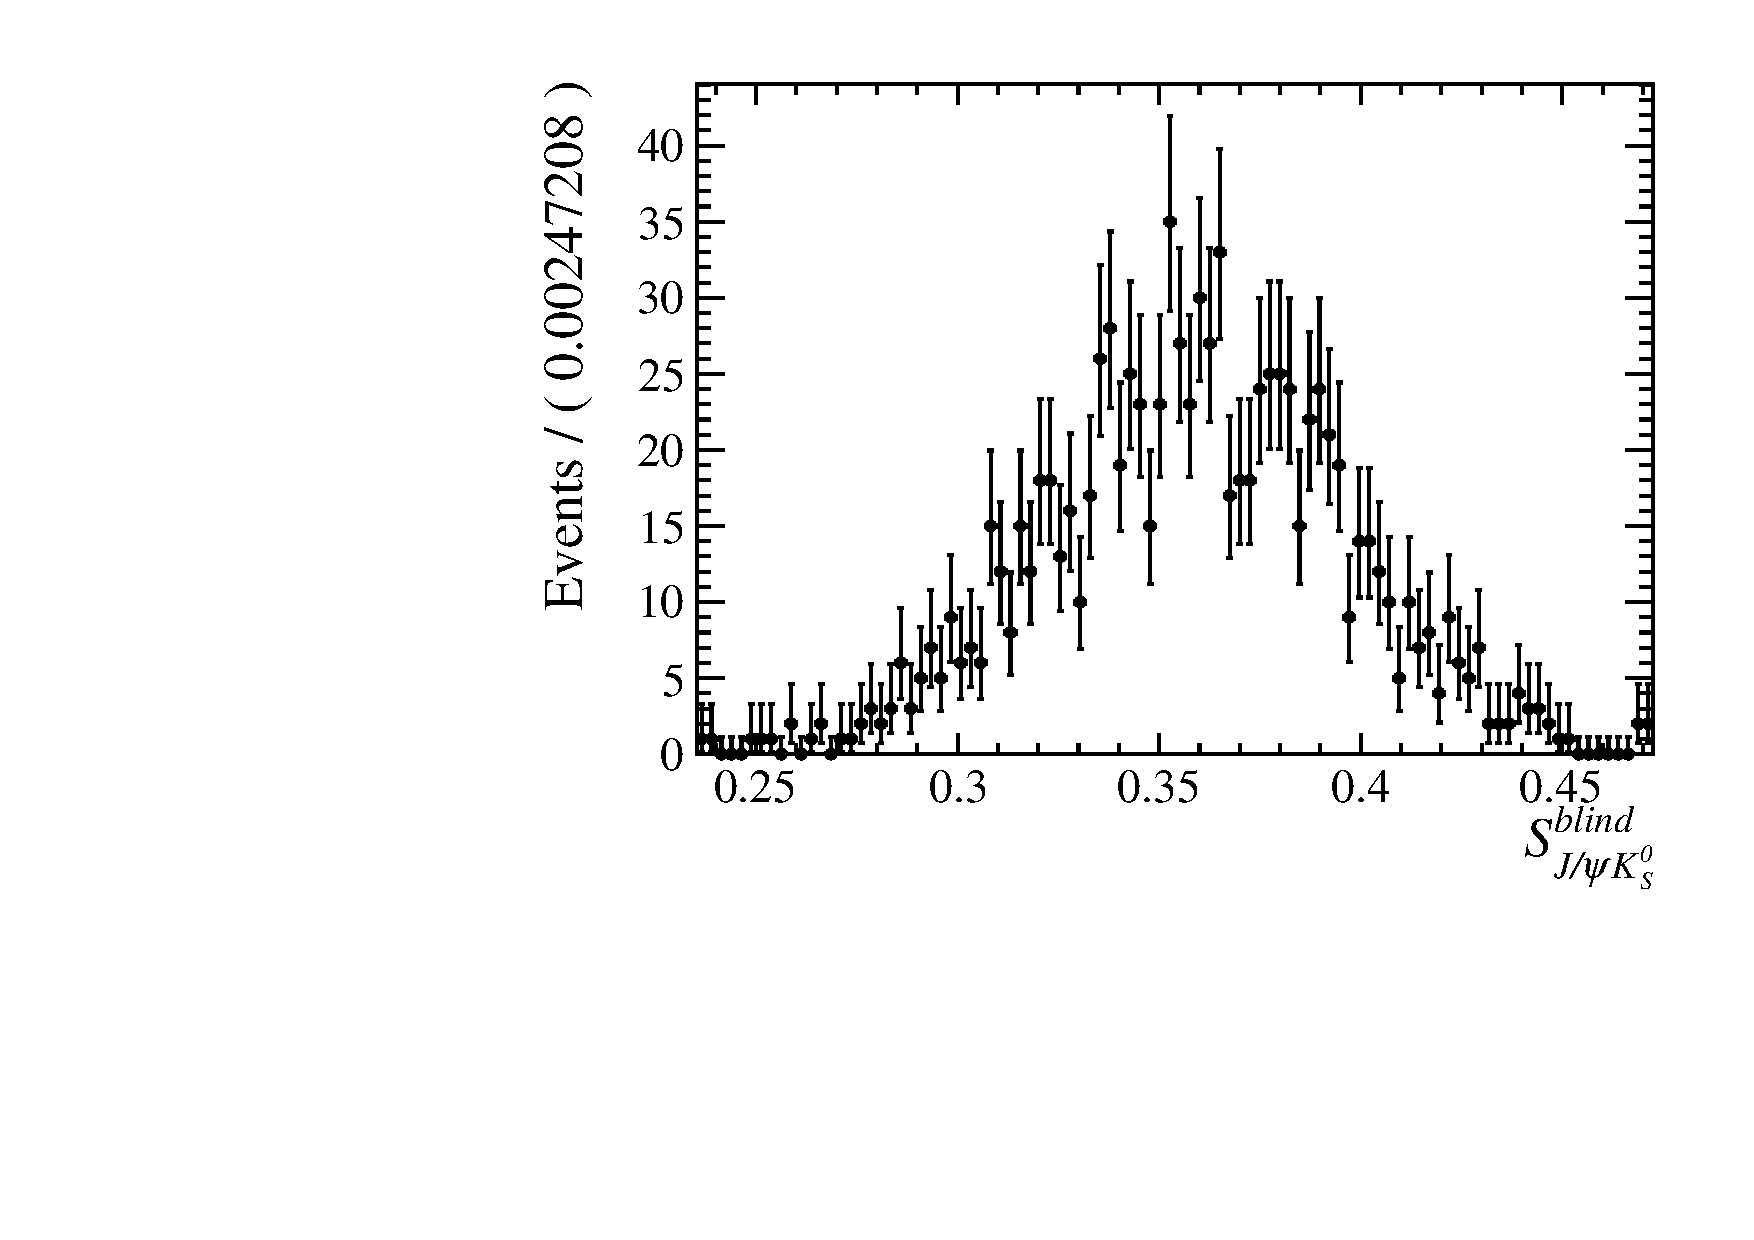
\includegraphics[width=0.48\textwidth]{private/content/measurement-of-sin2beta/figs/bootstrapping_parSigTimeSin2b_blind.pdf}
\hfill
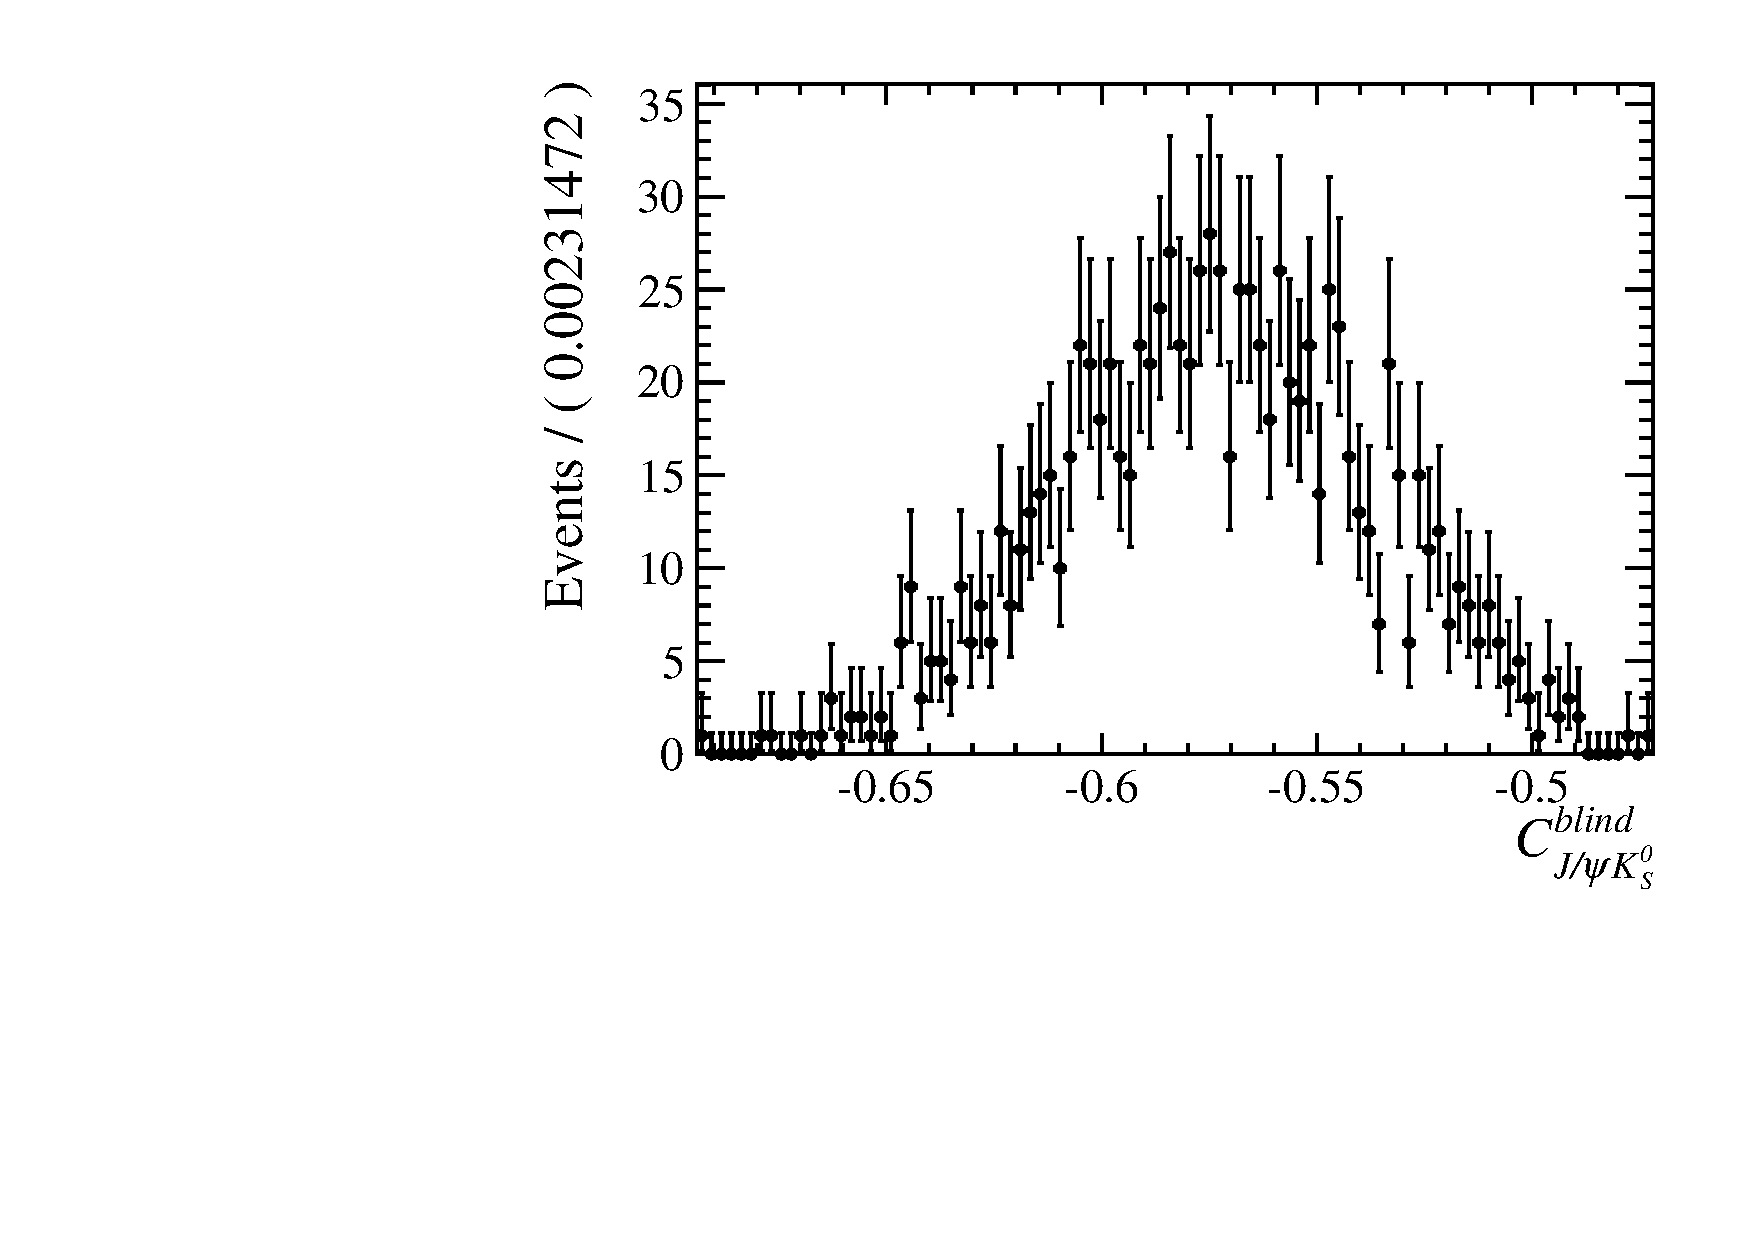
\includegraphics[width=0.48\textwidth]{private/content/measurement-of-sin2beta/figs/bootstrapping_parSigTimeCjpsiKS_blind.pdf}
\caption{
Parameter distributions for \SJpsiKS and \CJpsiKS from $\num{960}$
bootstrapping iterations of the \sPlot fit.}
\label{fig:measurement_of_sin2beta:systematics:cross_checks:splot_fit:bootstrapping}
\end{figure}

%------------------------------------------------------------------------------%
\subsubsection{Subsamples}
\label{sec:measurement_of_sin2beta:systematics:cross_checks:subsamples}
%
To check for possible systematic effects, fits in different subsamples of the
nominal data set are conducted. The cross-checks are performed in categories of
track type (\catDD \vs \catLL), trigger requirement (\catAU \vs \catEB), tagging
algorithm (\catOS \vs \catSS \vs \catBS), magnet polarity (Up \vs Down), and
admixtures of those together with the year of data-taking (\catOO \vs \catOT).
As a control sample the full data set is also split randomly into five disjoint
subsets (Rndm1-5). \Cref{fig:measurement_of_sin2beta:systematics:cross_checks:subsamples:s_and_c}
illustrates the outcome. No significant deviation is present.
%
\begin{figure}
\centering
%!TEX root = ../main.tex

\definecolor{Black}{HTML}{000000}
\definecolor{Red}{HTML}{FC5716}

\colorlet{ClrRndm}{Black}
\colorlet{ClrTrigger}{Black}
\colorlet{ClrTagger}{Black}
\colorlet{ClrYear}{Black}
\colorlet{ClrYearTagger}{Black}
\colorlet{ClrTrack}{Black}
\colorlet{ClrFullFit}{Red}
\colorlet{ClrUncert}{Red!40}

\begin{tikzpicture}[
  exp_label/.style={
    anchor=west,
    %minimum width=10em,
    align=left,
    font=\small\sffamily,
    inner sep=0.5em,
    outer sep=0,
  },
  exp_result/.style={
    anchor=east,
    align=right,
    font=\footnotesize\sffamily,
    inner sep=0.5em,
    outer sep=0,
    yshift=0.22em
  }
]
\begin{axis}[
  width=\textwidth,
  height=65ex,
  font=\small,
  xmin=0.1,xmax=1.1,ymin=0.3,ymax=23.7,
  xlabel={$\SJpsiKS$},
  xlabel style={
        at={(ticklabel cs:1)},
        anchor=north east,
    },%
  xtick={0.3, 0.4, 0.5, 0.6, 0.7, 0.8, 0.9, 1.0},
  % xticklabels={,,},
  xticklabel style={%
    major tick length=3pt
  },
  hide y axis
]

\begin{pgfonlayer}{background}
% line at 0
% \draw[ultra thin,color=Black!80]({rel axis cs:0,0}-|{axis cs:0,0}) -- ({rel axis cs:0,1}-|{axis cs:0,0});
% line at -1
% \draw[ultra thin,color=Black!80,dashed]({rel axis cs:0,0}-|{axis cs:-1,0}) -- ({rel axis cs:-1,1}-|{axis cs:-1,0});
% line at +1
% \draw[ultra thin,color=Black!80,dashed]({rel axis cs:0,0}-|{axis cs:+1,0}) -- ({rel axis cs:+1,1}-|{axis cs:+1,0});
% filled area at average value
\fill[color=ClrUncert] ({rel axis cs:0,0}-|{axis cs:0.693724977,0}) rectangle ({rel axis cs:0.763116749,1}-|{axis cs:0.763116749,0});
% line at average value
\draw[ultra thin,color=ClrFullFit]({rel axis cs:0,0}-|{axis cs:0.7285040271,0}) -- ({rel axis cs:0.7285040271,1}-|{axis cs:0.7285040271,0});

% lines to separate the different subsamples categories
\draw[ultra thin, dashed, color=Black!80] (axis cs: \pgfkeysvalueof{/pgfplots/xmin},18.5) -- (axis cs: \pgfkeysvalueof{/pgfplots/xmax},18.5);
\draw[ultra thin, dashed, color=Black!80] (axis cs: \pgfkeysvalueof{/pgfplots/xmin},16.5) -- (axis cs: \pgfkeysvalueof{/pgfplots/xmax},16.5);
\draw[ultra thin, dashed, color=Black!80] (axis cs: \pgfkeysvalueof{/pgfplots/xmin},13.5) -- (axis cs: \pgfkeysvalueof{/pgfplots/xmax},13.5);
\draw[ultra thin, dashed, color=Black!80] (axis cs: \pgfkeysvalueof{/pgfplots/xmin},11.5) -- (axis cs: \pgfkeysvalueof{/pgfplots/xmax},11.5);
\draw[ultra thin, dashed, color=Black!80] (axis cs: \pgfkeysvalueof{/pgfplots/xmin}, 9.5) -- (axis cs: \pgfkeysvalueof{/pgfplots/xmax}, 9.5);
\draw[ultra thin, dashed, color=Black!80] (axis cs: \pgfkeysvalueof{/pgfplots/xmin}, 7.5) -- (axis cs: \pgfkeysvalueof{/pgfplots/xmax}, 7.5);
\draw[ultra thin, dashed, color=Black!80] (axis cs: \pgfkeysvalueof{/pgfplots/xmin}, 1.5) -- (axis cs: \pgfkeysvalueof{/pgfplots/xmax}, 1.5);
\end{pgfonlayer}

%-------------------------------------------------------------------------------
% Random
\node[exp_label, color=ClrRndm] (Rndm1_lbl) at (axis cs: \pgfkeysvalueof{/pgfplots/xmin},23){Rndm1};
\node[exp_label, color=ClrRndm] (Rndm2_lbl) at (axis cs: \pgfkeysvalueof{/pgfplots/xmin},22){Rndm2};
\node[exp_label, color=ClrRndm] (Rndm3_lbl) at (axis cs: \pgfkeysvalueof{/pgfplots/xmin},21){Rndm3};
\node[exp_label, color=ClrRndm] (Rndm4_lbl) at (axis cs: \pgfkeysvalueof{/pgfplots/xmin},20){Rndm4};
\node[exp_label, color=ClrRndm] (Rndm5_lbl) at (axis cs: \pgfkeysvalueof{/pgfplots/xmin},19){Rndm5};


% Full uncertainty
\addplot+[only marks,
    thin,
    solid,
    color = ClrRndm,
    mark=*,
    mark options={%
      scale=0.7,
      draw=ClrRndm
    },
    error bars/.cd,
    x dir=both, x explicit,
    y dir=both, y explicit,
    error mark options={%
      rotate=90,
      mark size=3pt,
      color=ClrRndm
    }
]
table[
        x error plus=ex+,
        x error minus=ex-,
]{
  x             y  ex+            ex-  
  0.7712377343  23 0.073430739    0.074585294
  0.7008958291  22 0.07418394334  0.07429740627
  0.6470130176  21 0.0762116547   0.07704696965
  0.8668497014  20 0.078519274    0.07990252538
  0.6722234942  19 0.07662743282  0.0767069747
};

%-------------------------------------------------------------------------------
% Trigger
\node[exp_label, color=ClrTrigger] (AU_lbl) at (axis cs: \pgfkeysvalueof{/pgfplots/xmin},18){Almost unbiased};
\node[exp_label, color=ClrTrigger] (EB_lbl) at (axis cs: \pgfkeysvalueof{/pgfplots/xmin},17){Exclusively biased};


% Full uncertainty
\addplot+[only marks,
    thin,
    solid,
    color = ClrTrigger,
    mark=*,
    mark options={%
      scale=0.7,
      draw=ClrTrigger
    },
    error bars/.cd,
    x dir=both, x explicit,
    y dir=both, y explicit,
    error mark options={%
      rotate=90,
      mark size=3pt,
      color=ClrTrigger
    }
]
table[
        x error plus=ex+,
        x error minus=ex-,
]{
  x            y   ex+            ex-  
  0.710745651  18  0.03795927938  0.03833662133
  0.8250789821 17  0.08032890424  0.08135593581
};

%-------------------------------------------------------------------------------
% Tagger
\node[exp_label, color=ClrTagger] (OS_lbl) at (axis cs: \pgfkeysvalueof{/pgfplots/xmin},16){Excl. OS};
\node[exp_label, color=ClrTagger] (SS_lbl) at (axis cs: \pgfkeysvalueof{/pgfplots/xmin},15){Excl. SS};
\node[exp_label, color=ClrTagger] (OL_lbl) at (axis cs: \pgfkeysvalueof{/pgfplots/xmin},14){Excl. BS};


% Full uncertainty
\addplot+[only marks,
    thin,
    solid,
    color = ClrTagger,
    mark=*,
    mark options={%
      scale=0.7,
      draw=ClrTagger
    },
    error bars/.cd,
    x dir=both, x explicit,
    y dir=both, y explicit,
    error mark options={%
      rotate=90,
      mark size=3pt,
      color=ClrTagger
    }
]
table[
        x error plus=ex+,
        x error minus=ex-,
]{
  x             y   ex+            ex-  
  0.7288118238  16  0.04027423794  0.04031385447
  0.6422124342  15  0.1142810315   0.1140158165
  0.7777873414  14  0.08196002749  0.0831860115
};

%-------------------------------------------------------------------------------
% Year
\node[exp_label, color=ClrYear] (11OS_lbl) at (axis cs: \pgfkeysvalueof{/pgfplots/xmin},13){2011};
\node[exp_label, color=ClrYear] (11SS_lbl) at (axis cs: \pgfkeysvalueof{/pgfplots/xmin},12){2012};

% Full uncertainty
\addplot+[only marks,
    thin,
    solid,
    color = ClrYear,
    mark=*,
    mark options={%
      scale=0.7,
      draw=ClrYear
    },
    error bars/.cd,
    x dir=both, x explicit,
    y dir=both, y explicit,
    error mark options={%
      rotate=90,
      mark size=3pt,
      color=ClrYear
    }
]
table[
        x error plus=ex+,
        x error minus=ex-,
]{
  x            y  ex+            ex-  
  0.6268677992 13 0.06008359319  0.06057614937
  0.7765020167 12 0.04163076047  0.0417892058
};

%-------------------------------------------------------------------------------
% Track type
\node[exp_label, color=ClrTrack] (11DD_lbl) at (axis cs: \pgfkeysvalueof{/pgfplots/xmin},11){downstream};
\node[exp_label, color=ClrTrack] (11LL_lbl) at (axis cs: \pgfkeysvalueof{/pgfplots/xmin},10){long};


% Full uncertainty
\addplot+[only marks,
    thin,
    solid,
    color = ClrTrack,
    mark=*,
    mark options={%
      scale=0.7,
      draw=ClrTrack
    },
    error bars/.cd,
    x dir=both, x explicit,
    y dir=both, y explicit,
    error mark options={%
      rotate=90,
      mark size=3pt,
      color=ClrTrack
    }
]
table[
        x error plus=ex+,
        x error minus=ex-,
]{
  x            y  ex+            ex-  
  0.7509159107 11 0.04218332052  0.0424135402
  0.6846890918 10 0.05867667758  0.05950751898
};

%-------------------------------------------------------------------------------
% Magnet polarity and Year
\node[exp_label, color=ClrYearTagger] (11UP_lbl) at (axis cs: \pgfkeysvalueof{/pgfplots/xmin},9){Up};
\node[exp_label, color=ClrYearTagger] (11DW_lbl) at (axis cs: \pgfkeysvalueof{/pgfplots/xmin},8){Down};


% Full uncertainty
\addplot+[only marks,
    thin,
    solid,
    color = ClrYearTagger,
    mark=*,
    mark options={%
      scale=0.7,
      draw=ClrYearTagger
    },
    error bars/.cd,
    x dir=both, x explicit,
    y dir=both, y explicit,
    error mark options={%
      rotate=90,
      mark size=3pt,
      color=ClrYearTagger
    }
]
table[
        x error plus=ex+,
        x error minus=ex-,
]{
  x            y  ex+            ex-  
  0.763932558  9  0.05054925972  0.05095339912
  0.6973324655 8  0.0463213394   0.04667624179
};

%-------------------------------------------------------------------------------
% Year and Tagger
\node[exp_label, color=ClrYearTagger] (11OS_lbl) at (axis cs: \pgfkeysvalueof{/pgfplots/xmin},7){11 Excl. OS};
\node[exp_label, color=ClrYearTagger] (11SS_lbl) at (axis cs: \pgfkeysvalueof{/pgfplots/xmin},6){11 Excl. SS};
\node[exp_label, color=ClrYearTagger] (11BS_lbl) at (axis cs: \pgfkeysvalueof{/pgfplots/xmin},5){11 Excl. BS};
\node[exp_label, color=ClrYearTagger] (12OS_lbl) at (axis cs: \pgfkeysvalueof{/pgfplots/xmin},4){12 Excl. OS};
\node[exp_label, color=ClrYearTagger] (12SS_lbl) at (axis cs: \pgfkeysvalueof{/pgfplots/xmin},3){12 Excl. SS};
\node[exp_label, color=ClrYearTagger] (12BS_lbl) at (axis cs: \pgfkeysvalueof{/pgfplots/xmin},2){12 Excl. BS};

% Full uncertainty
\addplot+[only marks,
    thin,
    solid,
    color = ClrYearTagger,
    mark=*,
    mark options={%
      scale=0.7,
      draw=ClrYearTagger
    },
    error bars/.cd,
    x dir=both, x explicit,
    y dir=both, y explicit,
    error mark options={%
      rotate=90,
      mark size=3pt,
      color=ClrYearTagger
    }
]
table[
        x error plus=ex+,
        x error minus=ex-,
]{
  x            y  ex+            ex-  
  0.6065272082 7  0.06982395205  0.07056593733
  0.5470900868 6  0.1983877985   0.1995795379
  0.766496126  5  0.1417018624   0.1464811229
  0.7878244056 4  0.04842544413  0.04880814202
  0.686046884  3  0.1358504128   0.1356937662
  0.7839887379 2  0.09580978913  0.09899488064
};

%-------------------------------------------------------------------------------
% Full Fit
\node[exp_label, color=ClrFullFit] (Average_lbl) at (axis cs: \pgfkeysvalueof{/pgfplots/xmin},1)  
{Nominal fit};

% Full uncertainty
\addplot+[only marks,
    thin,
    solid, 
    color = ClrFullFit,
    mark=none,
    mark options={%
      scale=0.7,
      draw=ClrFullFit
    },
    error bars/.cd,
    x dir=both, x explicit,
    y dir=both, y explicit,
    error mark options={%
      rotate=90,
      mark size=3pt,
      color=ClrFullFit
    }
]
table[
        x error plus=ex+,
        x error minus=ex-,
]{
  x            y  ex+            ex-
  0.7285040271 1  0.03461272157  0.03477905032
};

\end{axis}
\end{tikzpicture}

%!TEX root = ../main.tex

\definecolor{Black}{HTML}{000000}
\definecolor{Red}{HTML}{FC5716}

\colorlet{ClrRndm}{Black}
\colorlet{ClrTrigger}{Black}
\colorlet{ClrTagger}{Black}
\colorlet{ClrTaggerYear}{Black}
\colorlet{ClrMagnetYear}{Black}
\colorlet{ClrTrackYear}{Black}
\colorlet{ClrFullFit}{Red}
\colorlet{ClrUncert}{Red!40}

\begin{tikzpicture}[
  exp_label/.style={
    anchor=west,
    %minimum width=10em,
    align=left,
    font=\small\sffamily,
    inner sep=0.5em,
    outer sep=0,
  },
  exp_result/.style={
    anchor=east,
    align=right,
    font=\footnotesize\sffamily,
    inner sep=0.5em,
    outer sep=0,
    yshift=0.22em
  }
]
\begin{axis}[
  width=\textwidth,
  height=65ex,
  font=\small,
  xmin=-0.661638482,xmax=0.338361518,ymin=0.3,ymax=23.7,
  xlabel={$\CJpsiKS$},
  xlabel style={
        at={(ticklabel cs:1)},
        anchor=north east,
    },%
  xtick={-0.4, -0.3, -0.2, -0.1, 0, 0.1, 0.2, 0.3},
  % xticklabels={,,},
  xticklabel style={%
    major tick length=3pt
  },
  hide y axis
]

\begin{pgfonlayer}{background}
% line at 0
% \draw[ultra thin,color=Black!80]({rel axis cs:0,0}-|{axis cs:0,0}) -- ({rel axis cs:0,1}-|{axis cs:0,0});
% line at -1
% \draw[ultra thin,color=Black!80,dashed]({rel axis cs:0,0}-|{axis cs:-1,0}) -- ({rel axis cs:-1,1}-|{axis cs:-1,0});
% line at +1
% \draw[ultra thin,color=Black!80,dashed]({rel axis cs:0,0}-|{axis cs:+1,0}) -- ({rel axis cs:+1,1}-|{axis cs:+1,0});
% filled area at average value
\fill[color=ClrUncert] ({rel axis cs:0,0}-|{axis cs:-0.06526549,0}) rectangle ({rel axis cs:-0.001013543,1}-|{axis cs:-0.001013543,0});
% line at average value
\draw[ultra thin,color=ClrFullFit]({rel axis cs:0,0}-|{axis cs:-0.0331344551,0}) -- ({rel axis cs:-0.0331344551,1}-|{axis cs:-0.0331344551,0});

% lines to separate the different subsamples categories
\draw[ultra thin, dashed, color=Black!80] (axis cs: \pgfkeysvalueof{/pgfplots/xmin},18.5) -- (axis cs: \pgfkeysvalueof{/pgfplots/xmax},18.5);
\draw[ultra thin, dashed, color=Black!80] (axis cs: \pgfkeysvalueof{/pgfplots/xmin},16.5) -- (axis cs: \pgfkeysvalueof{/pgfplots/xmax},16.5);
\draw[ultra thin, dashed, color=Black!80] (axis cs: \pgfkeysvalueof{/pgfplots/xmin},13.5) -- (axis cs: \pgfkeysvalueof{/pgfplots/xmax},13.5);
\draw[ultra thin, dashed, color=Black!80] (axis cs: \pgfkeysvalueof{/pgfplots/xmin},11.5) -- (axis cs: \pgfkeysvalueof{/pgfplots/xmax},11.5);
\draw[ultra thin, dashed, color=Black!80] (axis cs: \pgfkeysvalueof{/pgfplots/xmin}, 9.5) -- (axis cs: \pgfkeysvalueof{/pgfplots/xmax}, 9.5);
\draw[ultra thin, dashed, color=Black!80] (axis cs: \pgfkeysvalueof{/pgfplots/xmin}, 7.5) -- (axis cs: \pgfkeysvalueof{/pgfplots/xmax}, 7.5);
\draw[ultra thin, dashed, color=Black!80] (axis cs: \pgfkeysvalueof{/pgfplots/xmin}, 1.5) -- (axis cs: \pgfkeysvalueof{/pgfplots/xmax}, 1.5);
\end{pgfonlayer}

%-------------------------------------------------------------------------------
% Random
\node[exp_label, color=ClrRndm] (Rndm1_lbl) at (axis cs: \pgfkeysvalueof{/pgfplots/xmin},23){Rndm1};
\node[exp_label, color=ClrRndm] (Rndm2_lbl) at (axis cs: \pgfkeysvalueof{/pgfplots/xmin},22){Rndm2};
\node[exp_label, color=ClrRndm] (Rndm3_lbl) at (axis cs: \pgfkeysvalueof{/pgfplots/xmin},21){Rndm3};
\node[exp_label, color=ClrRndm] (Rndm4_lbl) at (axis cs: \pgfkeysvalueof{/pgfplots/xmin},20){Rndm4};
\node[exp_label, color=ClrRndm] (Rndm5_lbl) at (axis cs: \pgfkeysvalueof{/pgfplots/xmin},19){Rndm5};


% Full uncertainty
\addplot+[only marks,
    thin,
    solid,
    color = ClrRndm,
    mark=*,
    mark options={%
      scale=0.7,
      draw=ClrRndm
    },
    error bars/.cd,
    x dir=both, x explicit,
    y dir=both, y explicit,
    error mark options={%
      rotate=90,
      mark size=3pt,
      color=ClrRndm
    }
]
table[
        x error plus=ex+,
        x error minus=ex-,
]{
  x             y  ex+            ex-  
  0.02558441126 23 0.07021323593  0.07052451479
 -0.02565350348 22 0.07032629746  0.07023613489
 -0.06004908338 21 0.07253280748  0.07258763226
  0.04845072951 20 0.07425395458  0.07438156378
 -0.1428659543  19 0.07206119305  0.07164963211
};

%-------------------------------------------------------------------------------
% Trigger
\node[exp_label, color=ClrTrigger] (AU_lbl) at (axis cs: \pgfkeysvalueof{/pgfplots/xmin},18){Almost unbiased};
\node[exp_label, color=ClrTrigger] (EB_lbl) at (axis cs: \pgfkeysvalueof{/pgfplots/xmin},17){Exclusively biased};


% Full uncertainty
\addplot+[only marks,
    thin,
    solid,
    color = ClrTrigger,
    mark=*,
    mark options={%
      scale=0.7,
      draw=ClrTrigger
    },
    error bars/.cd,
    x dir=both, x explicit,
    y dir=both, y explicit,
    error mark options={%
      rotate=90,
      mark size=3pt,
      color=ClrTrigger
    }
]
table[
        x error plus=ex+,
        x error minus=ex-,
]{
  x             y  ex+            ex-  
 -0.05724869114 18 0.0348958308   0.03505910715
  0.1135758275  17 0.08424427739  0.08455088326
};

%-------------------------------------------------------------------------------
% Tagger
\node[exp_label, color=ClrTagger] (OS_lbl) at (axis cs: \pgfkeysvalueof{/pgfplots/xmin},16){Excl. OS};
\node[exp_label, color=ClrTagger] (SS_lbl) at (axis cs: \pgfkeysvalueof{/pgfplots/xmin},15){Excl. SS};
\node[exp_label, color=ClrTagger] (OL_lbl) at (axis cs: \pgfkeysvalueof{/pgfplots/xmin},14){Excl. BS};


% Full uncertainty
\addplot+[only marks,
    thin,
    solid,
    color = ClrTagger,
    mark=*,
    mark options={%
      scale=0.7,
      draw=ClrTagger
    },
    error bars/.cd,
    x dir=both, x explicit,
    y dir=both, y explicit,
    error mark options={%
      rotate=90,
      mark size=3pt,
      color=ClrTagger
    }
]
table[
        x error plus=ex+,
        x error minus=ex-,
]{
  x              y  ex+            ex-  
 -0.02182150859  16 0.03814187442  0.03797590581
 -0.1537951611   15 0.09971756852  0.100219264
 -0.003393348382 14 0.07641748829  0.07583334821
};

%-------------------------------------------------------------------------------
% Year
\node[exp_label, color=ClrTaggerYear] (11OS_lbl) at (axis cs: \pgfkeysvalueof{/pgfplots/xmin},13){2011};
\node[exp_label, color=ClrTaggerYear] (11SS_lbl) at (axis cs: \pgfkeysvalueof{/pgfplots/xmin},12){2012};

% Full uncertainty
\addplot+[only marks,
    thin,
    solid,
    color = ClrTaggerYear,
    mark=*,
    mark options={%
      scale=0.7,
      draw=ClrTaggerYear
    },
    error bars/.cd,
    x dir=both, x explicit,
    y dir=both, y explicit,
    error mark options={%
      rotate=90,
      mark size=3pt,
      color=ClrTaggerYear
    }
]
table[
        x error plus=ex+,
        x error minus=ex-,
]{
  x             y  ex+            ex-  
 -0.1377370909  13 0.0566527629   0.05670454656
  0.01779585578 12 0.03918441137  0.03919889162
};

%-------------------------------------------------------------------------------
% Track type
\node[exp_label, color=ClrTrackYear] (11DD_lbl) at (axis cs: \pgfkeysvalueof{/pgfplots/xmin},11){downstream};
\node[exp_label, color=ClrTrackYear] (11LL_lbl) at (axis cs: \pgfkeysvalueof{/pgfplots/xmin},10){long};


% Full uncertainty
\addplot+[only marks,
    thin,
    solid,
    color = ClrTrackYear,
    mark=*,
    mark options={%
      scale=0.7,
      draw=ClrTrackYear
    },
    error bars/.cd,
    x dir=both, x explicit,
    y dir=both, y explicit,
    error mark options={%
      rotate=90,
      mark size=3pt,
      color=ClrTrackYear
    }
]
table[
        x error plus=ex+,
        x error minus=ex-,
]{
  x              y ex+            ex-  
  0.02305527233 11 0.03990761127  0.03995817734
 -0.1348991135  10 0.05465942884  0.05464262893
};

%-------------------------------------------------------------------------------
% Magnet polarity and Year
\node[exp_label, color=ClrMagnetYear] (11UP_lbl) at (axis cs: \pgfkeysvalueof{/pgfplots/xmin},9){Up};
\node[exp_label, color=ClrMagnetYear] (11DW_lbl) at (axis cs: \pgfkeysvalueof{/pgfplots/xmin},8){Down};


% Full uncertainty
\addplot+[only marks,
    thin,
    solid,
    color = ClrMagnetYear,
    mark=*,
    mark options={%
      scale=0.7,
      draw=ClrMagnetYear
    },
    error bars/.cd,
    x dir=both, x explicit,
    y dir=both, y explicit,
    error mark options={%
      rotate=90,
      mark size=3pt,
      color=ClrMagnetYear
    }
]
table[
        x error plus=ex+,
        x error minus=ex-,
]{
  x             y  ex+            ex-  
 -0.02376582561 9  0.04758795926  0.04766667594
 -0.03958096368 8  0.04345994293  0.04349885924
};

%-------------------------------------------------------------------------------
% Year and Tagger
\node[exp_label, color=ClrYearTagger] (11OS_lbl) at (axis cs: \pgfkeysvalueof{/pgfplots/xmin},7){11 Excl. OS};
\node[exp_label, color=ClrYearTagger] (11SS_lbl) at (axis cs: \pgfkeysvalueof{/pgfplots/xmin},6){11 Excl. SS};
\node[exp_label, color=ClrYearTagger] (11BS_lbl) at (axis cs: \pgfkeysvalueof{/pgfplots/xmin},5){11 Excl. BS};
\node[exp_label, color=ClrYearTagger] (12OS_lbl) at (axis cs: \pgfkeysvalueof{/pgfplots/xmin},4){12 Excl. OS};
\node[exp_label, color=ClrYearTagger] (12SS_lbl) at (axis cs: \pgfkeysvalueof{/pgfplots/xmin},3){12 Excl. SS};
\node[exp_label, color=ClrYearTagger] (12BS_lbl) at (axis cs: \pgfkeysvalueof{/pgfplots/xmin},2){12 Excl. BS};

% Full uncertainty
\addplot+[only marks,
    thin,
    solid,
    color = ClrMagnetYear,
    mark=*,
    mark options={%
      scale=0.7,
      draw=ClrMagnetYear
    },
    error bars/.cd,
    x dir=both, x explicit,
    y dir=both, y explicit,
    error mark options={%
      rotate=90,
      mark size=3pt,
      color=ClrMagnetYear
    }
]
table[
        x error plus=ex+,
        x error minus=ex-,
]{
  x             y  ex+            ex-  
 -0.1416388853  7  0.06636570598  0.06650951901
 -0.2190836868  6  0.1798749598   0.1802323117
 -0.06927973414 5  0.1361005602   0.1364507049
  0.03692319471 4  0.04628104909  0.04632236703
 -0.1231213771  3  0.1193367706   0.1196054976
  0.02946883833 2 0.09129763057   0.09168226591
};

%-------------------------------------------------------------------------------
% Full Fit
\node[exp_label, color=ClrFullFit] (Average_lbl) at (axis cs: \pgfkeysvalueof{/pgfplots/xmin},1)  
{Nominal fit};

% Full uncertainty
\addplot+[only marks,
    thin,
    solid, 
    color = ClrFullFit,
    mark=none,
    mark options={%
      scale=0.7,
      draw=ClrFullFit
    },
    error bars/.cd,
    x dir=both, x explicit,
    y dir=both, y explicit,
    error mark options={%
      rotate=90,
      mark size=3pt,
      color=ClrFullFit
    }
]
table[
        x error plus=ex+,
        x error minus=ex-,
]{
  x            y  ex+            ex-
 -0.0331344551 1  0.03212091232  0.03213103531
};
\end{axis}
\end{tikzpicture}

\caption{
Comparison of fit results of \SJpsiKS and \CJpsiKS for fits on various
subsamples.}
\label{fig:measurement_of_sin2beta:systematics:cross_checks:subsamples:s_and_c}
\end{figure}

%------------------------------------------------------------------------------%
\subsubsection{Pure time-dependent and time-integrated fit}
\label{sec:measurement_of_sin2beta:systematics:cross_checks:time_integrated}

\missing{Pure time-dependent and time-integrated fit}

% ------------------------------------------------------------------------------
\subsection{Systematics}
\label{sec:measurement_of_sin2beta:systematics:systematics}

\missing{Introduction into systematics section}

%...............................................................................
\subsubsection{Fit model}
\label{sec:measurement_of_sin2beta:systematics:systematics:fit_model}

Background tagging asymmetry:
\cf \cref{sec:measurement_of_sin2beta:physic_backgrounds:tagging_asymmetries}
non-vanishing tagging asymmetries in the background candidates sample
\ToyMC to study effect of neglecting in fit
1000 samples generated with time-dependent asymmetries given in Fig. XX

%...............................................................................
\subsubsection{Flavour Tagging}
\label{sec:measurement_of_sin2beta:systematics:systematics:tagging}

%...............................................................................
\subsubsection{Decay time resolution}
\label{sec:measurement_of_sin2beta:systematics:systematics:resolution}

%...............................................................................
\subsubsection{Decay time acceptance}
\label{sec:measurement_of_sin2beta:systematics:systematics:acceptance}

%...............................................................................
\subsubsection{Production asymmetry, $z$-scale, \DMd, and \DG}
\label{sec:measurement_of_sin2beta:systematics:systematics:further_studies}

% ------------------------------------------------------------------------------
\subsection{Summary of systematic effects}
\label{sec:measurement_of_sin2beta:systematics:summary}
